\documentclass{beamer}

% Thème Beamer
\usetheme{Madrid}
\usecolortheme{seahorse}

% Packages utiles
\usepackage[utf8]{inputenc}
\usepackage[T1]{fontenc}
\usepackage{amsmath, amssymb, amsthm}
\usepackage{graphicx}
\usepackage{hyperref}
\usepackage{tikz}
\usepackage{pgfplots}

% Métadonnées
\title{Géométrie des Données et Apprentissage Machine}
\subtitle{Module 1 -- Introduction enrichie avec exercices}
\author{Youssef MESRI - MINES Paris - PSL}
\date{\today}

\begin{document}

% Page de titre
\begin{frame}
  \titlepage
\end{frame}

% Sommaire
\begin{frame}{Plan}
  \tableofcontents
\end{frame}


%================= MODULE 1 =================
\section{Module 1 : Introduction à la géométrie des données}

\begin{frame}{Module 1 : plan}
\begin{itemize}
  \item Notion de données en haute dimension
  \item Malédiction de la dimension et concentration de distances
  \item Variétés et distances géodésiques
  \item PCA
  \item Isomap
  \item Diffusion Maps
  \item t-SNE
  \item TP1 : Visualisation MNIST/Swiss Roll avec PCA, t-SNE, Isomap.
  \item TP2: Comparaison PCA / Isomap / Diffusion maps (scikit-learn, PyGSP).
\end{itemize}
\end{frame}
% ------------------ Section 1 ------------------
\section{Motivations}

\begin{frame}{Pourquoi une géométrie des données ?}
  \begin{itemize}
    \item Données modernes : images, sons, textes → espaces $\mathbb{R}^d$ avec $d \gg 1$.
    \item Pourtant, elles possèdent souvent une \textbf{structure intrinsèque} de faible dimension.
    \item \textbf{Idée clé} : les données sont souvent concentrées sur une \textbf{variété} de dimension intrinsèque $k \ll d$.
    \item Exemple : images de chiffres manuscrits (784 dimensions) mais proches d’une \textit{variété} de dimension \textit{beaucoup} plus petite $\approx 10$.
  \end{itemize}
\end{frame}

\begin{frame}{Explosion dimensionnelle : malédiction de la dimension}
  \begin{itemize}
    \item Lorsque la dimension $d$ augmente, le volume de l’espace croît \textbf{exponentiellement}.
    \item Dans un cube unité $[0,1]^d$, la majeure partie du volume se concentre près des \textbf{bords}.
    \item Les distances deviennent moins discriminantes :
  \end{itemize}
  \begin{block}{Illustration mathématique}
    Soient $n$ points tirés uniformément dans $[0,1]^d$. On définit :
    \begin{align*}
      d_{\min} &= \min_{i \neq j} \|x_i - x_j\|, \\
      d_{\max} &= \max_{i \neq j} \|x_i - x_j\|.
    \end{align*}
    On observe que :
    \[
      \lim_{d \to \infty} \frac{d_{\max} - d_{\min}}{d_{\min}} \to 0.
    \]
    \textbf{Conséquence :} toutes les distances deviennent presque égales !
  \end{block}
\end{frame}

\begin{frame}{Explosion dimensionnelle : la malédiction de la dimension (suite)}
\textbf{Intuition :} \newline
- Quand la dimension $d$ augmente, les points aléatoires dans $[0,1]^d$ deviennent « équidistants ».  \newline
- La distance entre points se concentre autour d'une valeur moyenne. \newline
- Cette perte de pouvoir discriminant est une des formes de la \textbf{malédiction de la dimension}. 
\end{frame}

% ================= Section : Concentration - preuve =================
\section{Concentration des distances : preuve par récurrence}

\begin{frame}{Mise en place}
  Deux points $x,y\in[0,1]^d$ i.i.d. uniformes. Définir la distance au carré :
  \[
    S_d := \|x-y\|_2^2 = \sum_{i=1}^d (x_i-y_i)^2 = \sum_{i=1}^d X_i,
  \]
  où $X_i$ sont i.i.d. copies de $X:=(U-V)^2$ avec $U,V\sim\mathcal U[0,1]$ indépendants.
  On montrera : $\mathbb E[S_d]=d\mu$, $\operatorname{Var}(S_d)=d\sigma^2$ et la dispersion relative $\to 0$.
\end{frame}

\begin{frame}{Cas $d=1$ : loi de la différence et moments}
  Posons $Z:=U-V$. Alors $Z\sim$ loi triangulaire sur $[-1,1]$ de densité $f_Z(z)=1-|z|$.  \\
  Comme $X=Z^2$ :
  \begin{align*}
    \mathbb E[X] &= \int_{-1}^1 z^2 (1-|z|)\,dz 
    = 2\int_0^1 z^2(1-z)\,dz = 2\Big(\tfrac{1}{3}-\tfrac{1}{4}\Big)=\tfrac{1}{6}, \\
    \mathbb E[X^2] &= \int_{-1}^1 z^4 (1-|z|)\,dz 
    = 2\int_0^1 z^4(1-z)\,dz = 2\Big(\tfrac{1}{5}-\tfrac{1}{6}\Big)=\tfrac{1}{15}.
  \end{align*}
  Donc $\mu=\mathbb E[X]=\tfrac{1}{6}$ et $\sigma^2=\operatorname{Var}(X)=\tfrac{1}{15}-\tfrac{1}{36}=\tfrac{7}{180}$.
\end{frame}

\begin{frame}{Vérification alternative (moments de l'uniforme)}
  \small
  Moments utiles pour $W\sim\mathcal U[0,1]$ : $\mathbb E[W]=\tfrac12,\ \mathbb E[W^2]=\tfrac13,\ \mathbb E[W^3]=\tfrac14,\ \mathbb E[W^4]=\tfrac15$.
  Avec indépendance de $U,V$ :
  \[\mathbb E[(U-V)^4]=2\mathbb E[U^4]-4\mathbb E[U^3]\mathbb E[V]+6\mathbb E[U^2]\mathbb E[V^2]-4\mathbb E[U]\mathbb E[V^3]=\tfrac{1}{15}.\]
  On retrouve donc $\mathbb E[X^2]=\tfrac{1}{15}$ et $\operatorname{Var}(X)=\tfrac{7}{180}$.
\end{frame}

\begin{frame}{Étape de récurrence (somme de i.i.d.)}
  Supposer vrai pour $d$ : $\mathbb E[S_d]=d\mu$, $\operatorname{Var}(S_d)=d\sigma^2$. Pour $d+1$ :
  \[
    S_{d+1}=S_d+X_{d+1} \Rightarrow \mathbb E[S_{d+1}]=(d+1)\mu,\quad \operatorname{Var}(S_{d+1})=(d+1)\sigma^2,
  \]
  par indépendance. Par récurrence simple, les formules valent pour tout $d\ge1$.
\end{frame}

\begin{frame}{Concentration relative et Chebyshev}
  Coefficient de variation :
  \[
    \frac{\sqrt{\operatorname{Var}(S_d)}}{\mathbb E[S_d]}=\frac{\sqrt{d\,\sigma^2}}{d\,\mu} = \frac{C}{\sqrt d},\quad C=\frac{\sqrt{\sigma^2}}{\mu}=6\sqrt{\tfrac{7}{180}}.
  \]
  \vspace{0.2cm}
  \textbf{Chebyshev :} pour tout $\varepsilon>0$,
  \[
    \Pr\big(|S_d-\mathbb E[S_d]|\ge \varepsilon\,\mathbb E[S_d]\big)\le \frac{\sigma^2}{\varepsilon^2\mu^2}\cdot\frac{1}{d} \xrightarrow[d\to\infty]{} 0.
  \]
  Donc \textbf{concentration relative} de $S_d$ autour de sa moyenne.
\end{frame}

\begin{frame}{Interprétation géométrique}
  \begin{itemize}
    \item $\mathbb E[S_d]=d/6$ croît linéairement en $d$ (donc $\mathbb E[\|x-y\|_2]\asymp \sqrt d$).
    \item L'écart-type est $\asymp \sqrt d$ aussi, mais \textbf{relativement} à la moyenne il vaut $O(1/\sqrt d)$.
    \item En grande dimension, les distances se ressemblent \textbf{relativement} : perte de pouvoir discriminant.
  \end{itemize}
\end{frame}
\begin{frame}{Distance dans le cube unité : mise en place}
Soient $x,y \in [0,1]^d$ deux points i.i.d. uniformes. \newline
\vspace{0.3cm}
\textbf{Définition :}  
\[
S_d = \|x-y\|_2^2 = \sum_{i=1}^d (x_i-y_i)^2.
\]
\textbf{Objectif :} Étudier la concentration de $S_d$ autour de son espérance quand $d \to \infty$.
\end{frame}

\begin{frame}{Cas $d=1$ : calcul des moments}
Soient $U,V \sim \mathcal{U}[0,1]$ indépendants. Posons $X=(U-V)^2$.  
\begin{itemize}
  \item Espérance : $\mathbb{E}[X]=\tfrac{1}{6}$.
  \item Moment d'ordre 4 : $\mathbb{E}[(U-V)^4]=\tfrac{1}{15}$.
  \item Variance : $\operatorname{Var}(X)=\tfrac{7}{180}.$
\end{itemize}
Donc $\mu = 1/6$, $\sigma^2 = 7/180$.
\end{frame}

\begin{frame}{Étape de récurrence}
Soient $X_1,\dots,X_d$ i.i.d. copies de $X$.  
\[
S_d = \sum_{i=1}^d X_i.
\]
Hypothèse de récurrence : $\mathbb{E}[S_d]=d\mu$, $\operatorname{Var}(S_d)=d\sigma^2$. \newline
\vspace{0.2cm}
Alors pour $d+1$ :
\[
S_{d+1}=S_d+X_{d+1}.
\]
Par indépendance :
\[
\mathbb{E}[S_{d+1}] = (d+1)\mu, \quad \operatorname{Var}(S_{d+1})=(d+1)\sigma^2.
\]
Donc la propriété est vraie pour tout $d$.
\end{frame}

\begin{frame}{Concentration relative}
\textbf{Coefficient de variation :}
\[
\frac{\sqrt{\operatorname{Var}(S_d)}}{\mathbb{E}[S_d]} = \frac{\sqrt{d\sigma^2}}{d\mu} = \frac{C}{\sqrt{d}},
\]
avec $C = \frac{\sqrt{\sigma^2}}{\mu} = 6\sqrt{\tfrac{7}{180}}.$ \newline
\vspace{0.3cm}
Donc l’écart relatif décroît comme $1/\sqrt{d}$. Les distances deviennent indiscernables en grande dimension.
\end{frame}

\begin{frame}{Application de l’inégalité de Chebyshev}
Pour tout $\varepsilon>0$ :
\[
\Pr\left( |S_d - \mathbb{E}[S_d]| \geq \varepsilon \mathbb{E}[S_d] \right) \leq \frac{\sigma^2}{\varepsilon^2\mu^2}\cdot \frac{1}{d}.
\]
\vspace{0.3cm}
Ainsi, la probabilité d’un écart relatif décroît en $1/d$.
\end{frame}

\begin{frame}{Interprétation géométrique}
\begin{itemize}
  \item La distance moyenne entre deux points est $\sim d/6$.
  \item L’écart-type est $\sim \sqrt{d}$.
  \item Donc les distances sont \textbf{concentrées autour d’une valeur moyenne}.
  \item Résultat : en grande dimension, \textbf{toutes les distances se ressemblent}. \newline
  \textit{Conséquence : difficulté pour les méthodes basées sur les distances (kNN, clustering, etc.)}.
\end{itemize}
\end{frame}

\begin{frame}{Exemple numérique : distances en haute dimension}
  \begin{itemize}
    \item Simulation : on génère $10^4$ points dans $[0,1]^d$.
    \item On calcule la distance moyenne $\bar{d}$ et son écart-type $\sigma_d$.
    \item Résultat : $\sigma_d/\bar{d} \to 0$ quand $d \to \infty$.
  \end{itemize}
  \begin{center}
    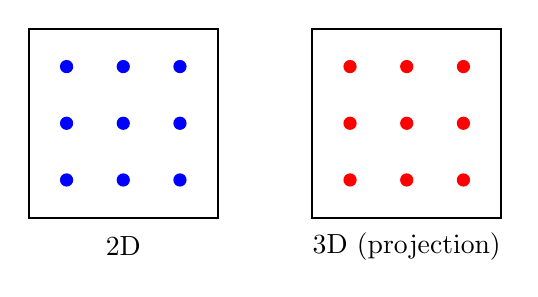
\begin{tikzpicture}[scale=1.2]
      % Points dans un carré 2D
      \draw[thick] (0,0) rectangle (2,2);
      \foreach \x in {0.4,1.0,1.6} {
        \foreach \y in {0.4,1.0,1.6} {
          \fill[blue] (\x,\y) circle (0.07);
        }
      }
      \node at (1,-0.3) {2D};
      % Points dans un cube 3D (projection)
      \begin{scope}[shift={(3,0)}]
        \draw[thick] (0,0) rectangle (2,2);
        \foreach \x in {0.4,1.0,1.6} {
          \foreach \y in {0.4,1.0,1.6} {
            \fill[red] (\x,\y) circle (0.07);
          }
        }
        \node at (1,-0.3) {3D (projection)};
      \end{scope}
    \end{tikzpicture}
    	iny Illustration : concentration des distances quand $d$ augmente (ici 2D et projection 3D).
  \end{center}
\end{frame}

\begin{frame}{Loi triangulaire de la différence de deux uniformes}
\textbf{Objectif :} Montrer que $Z = U - V$, avec $U,V\sim \mathcal U[0,1]$ i.i.d., suit une loi triangulaire sur $[-1,1]$.

\begin{block}{Convolution}
La densité de $Z$ est :
\[
  f_Z(z) = \int_{-\infty}^{+\infty} f_U(x) f_V(x-z) \, dx.
\]
Ici $f_U(x)=f_V(x)=1$ pour $x\in[0,1]$, 0 sinon.
\end{block}

\begin{itemize}
  \item Pour $z \in [-1,0]$ :
    \[f_Z(z) = \int_0^1 \mathbf{1}_{0 \le x-z \le 1} \, dx = \int_{0}^{1} \mathbf{1}_{z\le x \le 1+z} dx = 1+z.\]
  \item Pour $z \in [0,1]$ :
    \[f_Z(z) = \int_0^1 \mathbf{1}_{0 \le x-z \le 1} \, dx = \int_{z}^{1} dx = 1-z.\]
  \item Sinon $f_Z(z)=0$.
\end{itemize}

\begin{block}{Résultat}
\[
f_Z(z) = \begin{cases} 1+z, & -1\le z < 0, \\
1-z, & 0\le z \le 1, \\
0, & \text{sinon}.\end{cases}
\]
C’est une densité triangulaire, symétrique, avec maximum en $z=0$.
\end{block}

\begin{center}
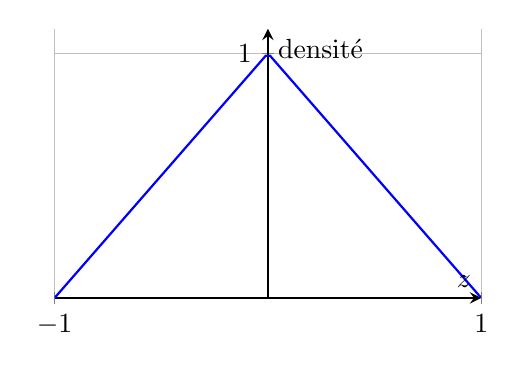
\begin{tikzpicture}
  \begin{axis}[
    width=7cm, height=5cm,
    axis lines=middle,
    xlabel={$z$}, ylabel={densité},
    xtick={-1,0,1}, ytick={0,1},
    domain=-1:1,
    samples=100,
    ymin=0, ymax=1.1,
    grid=major,
    thick
  ]
    \addplot[blue, thick] {1-abs(x)};
  \end{axis}
\end{tikzpicture}
\end{center}

\end{frame}

\begin{frame}{Exercice : loi de la différence}
Soient $U,V\sim \mathcal U[0,1]$ indépendants. Montrer que $Z=U-V$ a pour densité :
\[
f_Z(z) = \begin{cases} 1+z, & -1\le z<0, \\
1-z, & 0\le z\le 1, \\
0, & \text{sinon}.
\end{cases}\]

\textbf{Indication :} utiliser la convolution $f_Z(z)=\int f_U(x) f_V(x-z) dx$.
\end{frame}

\begin{frame}{Corrigé de l'exercice}
  \begin{itemize}
    \item Étape 1 : écrire $f_Z(z) = \int_{0}^{1} \mathbf{1}_{0\le x-z\le1} dx$.
    \item Étape 2 : séparer les cas $z<0$ et $z\ge0$.
    \item Étape 3 : calculer les intégrales :
      \[f_Z(z) = 1+z \text{ pour } z\in[-1,0],\quad f_Z(z)=1-z \text{ pour } z\in[0,1].\]
    \item Étape 4 : $f_Z(z)=0$ sinon.
  \end{itemize}
  On retrouve bien la loi triangulaire.
\end{frame}


\begin{frame}{Conséquences pratiques}
  \begin{itemize}
    \item Les méthodes classiques basées sur des distances euclidiennes deviennent inefficaces.
    \item Clustering et k-plus proches voisins perdent leur sens.
    \item Nécessité de méthodes tenant compte de la \textbf{structure intrinsèque} des données.
    \item D’où la géométrie des données : travailler dans une \textit{dimension intrinsèque} $k \ll d$.
  \end{itemize}
\end{frame}

\begin{frame}{Explosion dimensionnelle}
  \begin{itemize}
    \item Données modernes : images, sons, textes → espaces $\mathbb{R}^d$ avec $d \gg 1$.
    \item \textbf{Malédiction de la dimension} :
    \begin{itemize}
      \item Volume croît exponentiellement avec $d$.
      \item Distances deviennent peu discriminantes.
    \end{itemize}
  \item Besoin de méthodes exploitant la structure « cachée ».
  \end{itemize}
\end{frame}

\begin{frame}{Exemple : MNIST}
  \begin{itemize}
    \item Chaque image : $28 \times 28 = 784$ pixels → point dans $\mathbb{R}^{784}$.
    \item Mais les chiffres manuscrits vivent sur une structure de dimension \textbf{intrinsèque} $k \ll 784$.
    \item Question : comment trouver $k$ et représenter les données sur $\mathbb{R}^k$ ?
  \end{itemize}
\end{frame}

\begin{frame}{Exemple visuel : Swiss Roll}
  \begin{center}
    \includegraphics[width=0.6\textwidth]{swissroll.png} \\
    \tiny Un nuage de points en 3D mais structurellement 2D.
  \end{center}
\end{frame}

\begin{frame}{Idée clé}
  \begin{block}{Hypothèse de variété}
    Les données $x_i \in \mathbb{R}^d$ sont concentrées sur une variété $\mathcal{M}$ de dimension $k \ll d$.
  \end{block}
  \[
    x_i \in \mathcal{M} \subset \mathbb{R}^d, \quad \dim(\mathcal{M}) = k
  \]
\end{frame}

% ------------------ Section 2 ------------------
\section{Notions fondamentales}

\begin{frame}{Espace métrique}
  Un espace métrique est une paire $(X, d)$ avec :
  \begin{align*}
    d(x,y) &\geq 0 &\text{(positivité)} \\
    d(x,y) &= 0 \iff x=y &\text{(séparation)} \\
    d(x,y) &= d(y,x) &\text{(symétrie)} \\
    d(x,z) &\leq d(x,y) + d(y,z) &\text{(inégalité triangulaire)}
  \end{align*}
\end{frame}

\begin{frame}{Distances usuelles}
  \begin{itemize}
    \item Norme $\ell^2$: $d(x,y) = \|x-y\|_2 = \sqrt{\sum_i (x_i - y_i)^2}$.
    \item Norme $\ell^1$: $d(x,y) = \sum_i |x_i - y_i|$.
    \item Cosinus: $d(x,y) = 1 - \frac{\langle x, y \rangle}{\|x\| \|y\|}$.
    \item Distances adaptées aux graphes et variétés.
  \end{itemize}
\end{frame}

\begin{frame}{Distance cosinus et distance angulaire}
  Pour deux vecteurs $x,y \in \mathbb{R}^d$ non nuls :
  \[
    \cos\theta = \frac{x \cdot y}{\|x\|\|y\|}.
  \]

  \begin{itemize}
    \item \textbf{Distance cosinus classique :} 
      \[d_{\text{cos}}(x,y) = 1 - \cos\theta = 1 - \frac{x \cdot y}{\|x\|\|y\|}.\]
      - Varies entre 0 et 2.
      - Très utilisée en NLP et apprentissage automatique.
      - Pas une vraie métrique : triangle inequality peut échouer.

    \item \textbf{Distance basée sur l'angle :}
      \[d_{\text{angle}}(x,y) = \arccos\left(\frac{x \cdot y}{\|x\|\|y\|}\right).\]
      - Angle réel entre les vecteurs.
      - Vraie métrique : satisfait la triangle inequality.
      - Correspond à distance géodésique sur la sphère unité $S^{d-1}$.
  \end{itemize}

  %\begin{center}
  %  \includegraphics[width=0.2\textwidth]{cosine_vs_angle.png} \\
  %  \tiny Illustration : distance cosinus vs distance angulaire.
  %\end{center}
\end{frame}


\begin{frame}{Variété}
  \begin{itemize}
    \item Une variété $\mathcal{M}$ est un espace qui ressemble localement à $\mathbb{R}^k$.
    \item Exemple : sphère $S^2$ dans $\mathbb{R}^3$.
  \end{itemize}
  \begin{block}{Définition simplifiée}
    Pour chaque $x \in \mathcal{M}$, il existe un voisinage $U$ et une bijection $\varphi : U \to V \subset \mathbb{R}^k$.
  \end{block}
\end{frame}

\begin{frame}{Distance géodésique}
  Sur une variété $\mathcal{M}$, la distance naturelle est la longueur du plus court chemin $\gamma$ contenu dans $\mathcal{M}$ :
  \[
    d_\mathcal{M}(x,y) = \inf_{\gamma : [0,1]\to\mathcal{M}} \int_0^1 \|\dot{\gamma}(t)\| dt
  \]
  Exemple : distance sur la sphère = angle central multiplié par le rayon.
\end{frame}

\begin{frame}{Variétés de données : définition détaillée}
  \textbf{Définition informelle :} Une variété $\mathcal M$ de dimension $k$ est un sous-ensemble de $\mathbb R^d$ qui, localement autour de chaque point, ressemble à $\mathbb R^k$.

  \begin{itemize}
    \item Pour chaque point $x \in \mathcal M$, il existe un voisinage $U$ et une application bijective \textbf{carte} $\varphi: U \to V \subset \mathbb R^k$ telle que $\varphi$ et $\varphi^{-1}$ soient continues (ou différentiables pour les variétés différentiables).
    \item $k$ est la \textbf{dimension intrinsèque} de la variété.
    \item Exemple : le cercle $S^1 \subset \mathbb R^2$ est une variété 1D, la sphère $S^2 \subset \mathbb R^3$ est une variété 2D.
  \end{itemize}

  \textbf{Notation :} $\mathcal M^k \subset \mathbb R^d$ indique une variété de dimension $k$ dans $\mathbb R^d$.
\end{frame}

\begin{frame}{Propriétés fondamentales d'une variété}
  \begin{itemize}
    \item \textbf{Localement Euclidienne :} autour de chaque point, les distances et topologie se comportent comme dans $\mathbb R^k$.
    \item \textbf{Dimension intrinsèque :} le nombre minimal de coordonnées nécessaires pour paramétrer la variété.
    \item \textbf{Continuité et différentiabilité :} cartes et applications de transition doivent être continues ou différentiables.
    \item \textbf{Géodésiques :} la distance naturelle sur la variété est la longueur du plus court chemin restant dans la variété.
    \item \textbf{Courbure :} mesure locale de la déviation par rapport à un espace plat $\mathbb R^k$.
  \end{itemize}
\end{frame}

\begin{frame}{Exemples de variétés courantes}
  \begin{itemize}
    \item Cercle $S^1$ dans $\mathbb R^2$ (dimension 1).
    \item Sphère $S^2$ dans $\mathbb R^3$ (dimension 2).
    \item Cylindre dans $\mathbb R^3$ (dimension 2).
    \item Variétés de matrices de rang fixe : $\{X\in\mathbb R^{m\times n}: \mathrm{rank}(X)=r\}$.
    \item Espace des rotations $SO(3)$ (dimension 3), utilisé en robotique et vision.
  \end{itemize}
\end{frame}

\begin{frame}{Carte et atlas}
  \begin{itemize}
    \item \textbf{Carte :} fonction $\varphi: U\subset \mathcal M \to V\subset \mathbb R^k$ qui localement paramétrise la variété.
    \item \textbf{Atlas :} collection de cartes $\{(U_i,\varphi_i)\}$ recouvrant toute la variété.
    \item \textbf{Exemple :} sphère $S^2$, on peut utiliser coordonnées sphériques différentes pour couvrir les pôles et l'équateur.
    \item Les cartes permettent de définir des notions de dérivée, intégrale et courbure sur la variété.
  \end{itemize}
\end{frame}

\begin{frame}{Distances et géodésiques sur une variété}
  \begin{itemize}
    \item La distance euclidienne $\|x-y\|$ dans $\mathbb R^d$ ne respecte pas toujours la structure intrinsèque de la variété.
    \item La \textbf{distance géodésique} $d_\mathcal M(x,y)$ est la longueur du chemin le plus court restant dans la variété.
    \item Exemples :
      \begin{itemize}
        \item Cercle $S^1$: distance géodésique = arc le plus court entre deux points.
        \item Sphère $S^2$: distance géodésique = longueur de l'arc de grand cercle.
      \end{itemize}
    \item Les distances géodésiques sont fondamentales pour la réduction de dimension non linéaire et le clustering sur variétés.
  \end{itemize}
\end{frame}

\begin{frame}{Distance géodésique sur la sphère : arc de grand cercle}
%\begin{center}
%  \includegraphics[width=0.4\textwidth]{great_circle_arc.png} \\
%  \tiny Schéma : sphère de rayon $R$, points $A$ et $B$, grand cercle et angle $\theta$.
%\end{center}

\begin{itemize}
  \item Le plus court chemin sur la sphère est l'\textbf{arc de grand cercle} reliant $A$ et $B$.
  \item Longueur de l'arc : $L = R \cdot \theta$, avec $\theta$ en radians.
  \item Angle au centre : $\theta = \arccos\left(\frac{x \cdot y}{R^2}\right)$ pour $x,y \in S^2$.
  \item Pour une sphère unité ($R=1$) : $d_{S^2}(x,y) = \arccos(x \cdot y)$.
\end{itemize}
\end{frame}

\begin{frame}{Applications des variétés en science des données}
  \begin{itemize}
    \item Réduction de dimension non linéaire : Isomap, LLE, Diffusion Maps.
    \item Détection de structure intrinsèque dans des données haute dimension.
    \item Modélisation de données sur des espaces non Euclidiens : rotations, formes, graphes.
    \item Méthodes de machine learning adaptées aux données de faible dimension intrinsèque.
  \end{itemize}
\end{frame}

\begin{frame}{Laplacien de graphe}
  Pour un graphe $G=(V,E)$ avec poids $w_{ij}$ :
  \begin{align*}
    D_{ii} &= \sum_j w_{ij}, \\
    L &= D - W.
  \end{align*}
  Propriétés :
  \begin{itemize}
    \item $L$ est semi-défini positif.
    \item $L$ approxime le Laplacien sur la variété sous-jacente.
  \end{itemize}
\end{frame}

\begin{frame}{Exemple : chaleur sur un graphe}
  \[
    \frac{du}{dt} = -Lu
  \]
  $L$ joue le rôle de dérivée seconde discrète.
  Solution : $u(t) = e^{-tL}u(0)$.
\end{frame}

% ------------------ Section 3 ------------------
\section{Applications}

\begin{frame}{Réduction de dimension}
  But : trouver $f : \mathbb{R}^d \to \mathbb{R}^k$ qui conserve la géométrie.
  \begin{itemize}
    \item PCA : directions de variance maximale.
    \item Isomap : distances géodésiques.
    \item Diffusion maps : diffusion de chaleur.
  \end{itemize}
\end{frame}

\begin{frame}{PCA en formule}
  \begin{align*}
    \Sigma &= \frac{1}{n}\sum_{i=1}^n (x_i - \mu)(x_i - \mu)^T \\
    \text{vecteurs propres de } \Sigma &\Rightarrow directions principales.
  \end{align*}
\end{frame}

\begin{frame}{Analyse en Composantes Principales (PCA) : Introduction}
  \begin{itemize}
    \item PCA est une méthode linéaire de réduction de dimension.
    \item Objectif : trouver les directions principales (axes) qui capturent le plus de variance dans les données.
    \item Idée : projeter les données dans un sous-espace de dimension $k \ll d$ en minimisant la perte d'information.
    \item Utile pour visualisation, compression, prétraitement de machine learning.
  \end{itemize}
\end{frame}

\begin{frame}{Formulation mathématique de la PCA}
  \begin{itemize}
    \item Soient $X = [x_1, \dots, x_n]^\top \in \mathbb{R}^{n\times d}$ les données centrées ($\bar x = 0$).
    \item Matrice de covariance :
      \[\Sigma = \frac{1}{n} X^\top X \in \mathbb{R}^{d\times d}.\]
    \item Cherchons vecteurs propres $v_j$ et valeurs propres $\lambda_j$ :
      \[\Sigma v_j = \lambda_j v_j, \quad j=1,\dots,d.\]
    \item Les $v_j$ sont les directions principales (composantes principales).
  \end{itemize}
\end{frame}

\begin{frame}{Projection sur les composantes principales}
  \begin{itemize}
    \item Les $k$ premières composantes principales correspondent aux $k$ plus grandes valeurs propres $\lambda_1 \ge \lambda_2 \ge \dots \ge \lambda_k$.
    \item Projection :
      \[y_i = V_k^\top x_i, \quad V_k = [v_1, \dots, v_k] \in \mathbb{R}^{d\times k}.\]
    \item Reconstruction approchée :
      \[\hat{x}_i = V_k y_i = V_k V_k^\top x_i.\]
    \item Erreur de reconstruction : minimisée par la PCA.
  \end{itemize}
\end{frame}

\begin{frame}{Propriété d’optimalité}
  La PCA est l’approximation linéaire optimale au sens des moindres carrés :
  \[
    \min_{V_k \in \mathbb{R}^{d\times k}, V_k^\top V_k = I_k} \sum_{i=1}^n \|x_i - V_k V_k^\top x_i\|^2.\]
  
  La solution est donnée par les $k$ vecteurs propres associés aux $k$ plus grandes valeurs propres de $\Sigma$.
\end{frame}

\begin{frame}{Variance expliquée}
  \begin{itemize}
    \item Variance totale : $\mathrm{Tr}(\Sigma) = \sum_{j=1}^d \lambda_j$.
    \item Variance capturée par les $k$ premières composantes : $\sum_{j=1}^k \lambda_j$.
    \item Fraction de variance expliquée :
      \[
        \text{FVE}(k) = \frac{\sum_{j=1}^k \lambda_j}{\sum_{j=1}^d \lambda_j}.\]
    \item Permet de choisir le nombre optimal $k$ pour la réduction de dimension.
  \end{itemize}
\end{frame}

\begin{frame}{Exemple numérique}
  \begin{itemize}
    \item Données $X \in \mathbb{R}^{100\times 5}$ simulées.
    \item Calculer $\Sigma = X^\top X / 100$.
    \item Calcul des valeurs propres et vecteurs propres.
    \item Projection sur $k=2$ premières composantes principales pour visualisation.
    \item Observer la concentration des données le long des directions principales.
  \end{itemize}
\end{frame}

\begin{frame}{PCA et SVD}
  \begin{itemize}
    \item Alternative : utiliser la décomposition en valeurs singulières (SVD) : $X = U \Sigma V^\top$.
    \item Composantes principales : colonnes de $V$.
    \item Valeurs propres : carrés des valeurs singulières divisées par $n$.
    \item Utile pour $d \gg n$ ou pour stabilité numérique.
  \end{itemize}
\end{frame}

\begin{frame}{Exercice PCA}
  Soit un ensemble de données centrées $X \in \mathbb{R}^{10 \times 3}$ :
  \begin{itemize}
    \item Calculer la matrice de covariance $\Sigma$.
    \item Déterminer les vecteurs propres et valeurs propres.
    \item Projeter les données sur les 2 premières composantes principales.
  \end{itemize}
\end{frame}

\begin{frame}{Corrigé exercice PCA}
  \begin{itemize}
    \item Étape 1 : $\Sigma = X^\top X / 10$.
    \item Étape 2 : calcul des valeurs propres $\lambda_1 \ge \lambda_2 \ge \lambda_3$ et vecteurs propres $v_1,v_2,v_3$.
    \item Étape 3 : projection $y_i = [v_1,v_2]^\top x_i$.
    \item Étape 4 : visualisation et analyse de la variance expliquée.
  \end{itemize}
\end{frame}


\begin{frame}{Isomap}
  \begin{enumerate}
    \item Construire graphe $k$-NN.
    \item Approximer distances géodésiques par plus courts chemins.
    \item Appliquer MDS (multidimensional scaling).
  \end{enumerate}
\end{frame}

\begin{frame}{Isomap : Introduction}
  \begin{itemize}
    \item Isomap (Isometric Mapping) est une méthode non-linéaire de réduction de dimension.
    \item Objectif : préserver les distances géodésiques entre les points d’une variété plongée dans un espace de haute dimension.
    \item Extension de MDS (Multidimensional Scaling) aux variétés non-linéaires.
  \end{itemize}
\end{frame}

\begin{frame}{Idée clé d’Isomap}
  \begin{enumerate}
    \item Construire un graphe des plus proches voisins (k-NN ou $\epsilon$-voisinage).
    \item Approximater les distances géodésiques par des plus courts chemins dans le graphe.
    \item Appliquer le MDS classique avec ces distances géodésiques approximées.
  \end{enumerate}
\end{frame}

\begin{frame}{Étape 1 : Graphe de voisinage}
  \begin{itemize}
    \item Pour chaque point $x_i$, on relie ses $k$ plus proches voisins (ou tous les voisins dans une boule de rayon $\epsilon$).
    \item Arêtes pondérées par la distance euclidienne :
      \[ w_{ij} = \|x_i - x_j\|_2. \]
    \item Graphe $G=(V,E)$ approximant la structure locale de la variété.
  \end{itemize}
\end{frame}

\begin{frame}{Étape 2 : Distances géodésiques}
  \begin{itemize}
    \item La distance géodésique entre $x_i$ et $x_j$ est approximée par la longueur du plus court chemin dans $G$ :
      \[ d_G(i,j) = \min_{chemins(i \to j)} \sum_{(u,v)\in chemin} w_{uv}. \]
    \item Utilisation d’algorithmes classiques : Dijkstra ou Floyd–Warshall.
    \item Matrice des distances géodésiques $D_G = (d_G(i,j))_{i,j}$.
  \end{itemize}
\end{frame}

\begin{frame}{Étape 3 : Application de MDS}
  \begin{itemize}
    \item Objectif : trouver une configuration de points $Y_1, \ldots, Y_n \in \mathbb{R}^d$ telle que
      \
      \[ \|Y_i - Y_j\|^2 \approx d_G(i,j)^2. \]
    \item On applique le MDS classique (Scaling multidimensionnel) :
      
    \begin{enumerate}
      \item On construit la matrice des distances au carré $D_G^{(2)} = (d_G(i,j)^2)_{ij}$.
      \item On centre cette matrice :
        \
        \[ B = -\tfrac{1}{2} H D_G^{(2)} H, \quad H = I - \tfrac{1}{n} \mathbf{1}\mathbf{1}^\top. \]
      \item $B$ est une approximation de la matrice de Gram $YY^\top$.
      \item On diagonalise $B = V \Lambda V^\top$.
      \item Les coordonnées en dimension $d$ sont données par :
        \
        \[ Y = V_d \Lambda_d^{1/2}, \]
        où $V_d$ contiennent les $d$ vecteurs propres principaux et $\Lambda_d$ les $d$ plus grandes valeurs propres.
    \end{enumerate}
    \item Ainsi, on obtient une immersion en $d$ dimensions qui préserve au mieux les distances géodésiques.
  \end{itemize}
\end{frame}

\begin{frame}{Étape 3 : Application de MDS}
  \begin{itemize}
    \item On applique le MDS classique sur $D_G$ pour obtenir une représentation en basse dimension.
    \item Centrage double :
      \[ B = -\tfrac{1}{2} H D_G^{(2)} H, \quad H = I - \tfrac{1}{n} \mathbf{1}\mathbf{1}^\top. \]
    \item Décomposition spectrale :
      \[ B = V \Lambda V^\top. \]
    \item Coordonnées en dimension $d$ :
      \[ Y = V_d \Lambda_d^{1/2}. \]
  \end{itemize}
\end{frame}

\begin{frame}{Propriétés d’Isomap}
  \begin{itemize}
    \item Préserve la géométrie globale de la variété.
    \item Gère des données fortement non-linéaires (spirale, Swiss roll).
    \item Consistance théorique : converge vers la métrique de la variété quand $n\to \infty$.
    \item Sensible aux choix de $k$ ou $\epsilon$.
  \end{itemize}
\end{frame}

\begin{frame}{Exemple : Swiss Roll}
  \begin{itemize}
    \item Données 3D enroulées en spirale (« rouleau suisse »).
    \item PCA : incapacité à « dérouler » la structure.
    \item Isomap : reconstitue correctement la structure 2D sous-jacente.
  \end{itemize}
  \begin{center}
    \includegraphics[width=0.6\textwidth]{swiss_roll_isomap.png}
  \end{center}
\end{frame}

\begin{frame}{Exercice Isomap}
  \begin{itemize}
    \item Générer un jeu de données 3D de type Swiss roll.
    \item Construire le graphe $k$-NN avec $k=10$.
    \item Calculer les plus courts chemins (algorithme de Dijkstra).
    \item Appliquer MDS sur la matrice de distances.
    \item Visualiser la représentation 2D obtenue.
  \end{itemize}
\end{frame}

\begin{frame}{Corrigé Exercice Isomap}
  \begin{itemize}
    \item Étape 1 : génération des points $(x,y,z)$.
    \item Étape 2 : construction du graphe $k$-NN.
    \item Étape 3 : distances géodésiques via Dijkstra.
    \item Étape 4 : matrice $B$ et décomposition spectrale.
    \item Résultat : une carte 2D déroulant le Swiss roll.
  \end{itemize}
\end{frame}

\begin{frame}{Résumé intuitif d'Isomap}
  \begin{itemize}
    \item But : représenter les données dans un espace de dimension réduite $d$ (typiquement 2 ou 3).
    \item On calcule d'abord les distances géodésiques $d_G(i,j)$ entre points dans l'espace original (via le graphe de voisinage).
    \item Puis on cherche des points $Y_i \in \mathbb{R}^d$ tels que :
      \
      \[ \|Y_i - Y_j\| \approx d_G(i,j). \]
    \item Ainsi :
      \begin{itemize}
        \item Les distances locales sont respectées.
        \item La géométrie intrinsèque de la variété est préservée.
        \item On obtient une carte en basse dimension reflétant la structure réelle des données.
      \end{itemize}
    \item Différence clé avec PCA : Isomap ne se base pas uniquement sur les distances euclidiennes globales, mais sur les distances intrinsèques (géodésiques).
  \end{itemize}
\end{frame}

\begin{frame}{Diffusion Maps}
  \begin{itemize}
    \item Construire matrice de transition $P = D^{-1}W$.
    \item Valeurs propres $\lambda_1, \lambda_2, ...$ et vecteurs propres $\psi_i$.
    \item Représentation des données :
    \[
      x \mapsto (\lambda_1^t\psi_1(x), \dots, \lambda_k^t\psi_k(x))
    \]
  \end{itemize}
\end{frame}

% ----------------- Diffusion Maps (à insérer) -----------------
\begin{frame}{Diffusion Maps : introduction}
  \begin{itemize}
    \item Diffusion Maps (Coifman \& Lafon, 2006) : méthode spectrale non-linéaire de réduction de dimension.
    \item Idée : utiliser la dynamique de diffusion (marche aléatoire) sur le graphe de voisinage pour révéler la géométrie intrinsèque.
    \item Résultat : coordonnées multi-échelle (robustes au bruit et à l'échantillonnage irrégulier).
  \end{itemize}
\end{frame}

% Exemple de slide Diffusion Maps avec notations cohérentes

\begin{frame}{Diffusion Maps : idée générale}
 \begin{itemize}
    \item Construire un graphe de similarité entre les points (par ex. noyau gaussien).
    \item Normaliser la matrice de similarité $K$ pour obtenir une matrice de transition stochastique $P$ d'une marche aléatoire.
    \item Les puissances $P^t$ décrivent la diffusion des probabilités après $t$ pas.
    \item Les coordonnées réduites sont données par les vecteurs propres dominants de $P$ associés aux valeurs propres $\{ \lambda_k \}$.
  \end{itemize}
\end{frame}

\begin{frame}[fragile]{Pseudo-code : Diffusion Maps (notations corrigées)}
\begin{verbatim}
Entrée : Données {x_i}, paramètre $\epsilon$ (bande du noyau), dimension cible d, temps t.
1. Construire la matrice de similarité : $K(i,j) = \exp(-\|x_i - x_j\|^2 / \epsilon)$.
2. Normaliser : D(i,i) = somme_j K(i,j).
3. Matrice de transition : P = D^{-1} K.
4. Calcul spectral : trouver les paires (\lambda_k, \phi_k) avec P \phi_k = \lambda_k \phi_k.
5. Embedding diffusion à temps t : y_i = (\lambda_1^t \phi_1(i), ..., \lambda_d^t \phi_d(i)).
Sortie : Points {y_i} en dimension réduite.
\end{verbatim}
\end{frame}

\begin{frame}{Remarques sur les notations}
  \begin{itemize}
    \item $K$ : matrice de similarité (symétrique positive).
    \item $D$ : matrice diagonale des degrés $D(i,i) = \sum_j K(i,j)$.
    \item $P = D^{-1} K$ : matrice de transition stochastique (les lignes somment à 1).
    \item $(\lambda_k, \phi_k)$ : valeurs propres et vecteurs propres droits de $P$.
    \item L'embedding utilise les $d$ plus grandes valeurs propres (hors $\lambda_0 = 1$ trivial).
  \end{itemize}
\end{frame}

\begin{frame}{Construction : noyau à noyau gaussien}
  \begin{itemize}
    \item Noyau usuel (gaussien) :
      \[
        W_{ij} = \exp\!\Big(-\frac{\|x_i-x_j\|^2}{\varepsilon}\Big).
      \]
    \item $\varepsilon>0$ est la largeur du noyau (contrôle la localité).
    \item $W$ est souvent construit sur un graphe $k$-NN (matrice creuse) pour l'efficacité.
    \item Noter le rôle de la densité d'échantillonnage : $q_i=\sum_j W_{ij}$.
  \end{itemize}
\end{frame}

\begin{frame}{Normalisation : corriger la densité (paramètre $\alpha$)}
  \begin{itemize}
    \item Pour neutraliser l'effet d'une densité non uniforme, on normalise :
      \[
        \widetilde W_{ij} = \frac{W_{ij}}{(q_i q_j)^\alpha},\qquad \alpha\in[0,1].
      \]
    \item Interprétations pratiques :
      \begin{itemize}
        \item $\alpha=0$ : pas de correction (sensitif à la densité).
        \item $\alpha=1$ : corrige l'échantillonnage pour approcher le Laplace–Beltrami (annule l'effet de densité).
        \item $\alpha\in(0,1)$ : compromis ; souvent $\alpha=1/2$ est utilisé empirique.
      \end{itemize}
    \item Ensuite : construire $\widetilde D=\mathrm{diag}(\widetilde d_i)$ avec $\widetilde d_i=\sum_j\widetilde W_{ij}$.
  \end{itemize}
\end{frame}

\begin{frame}{Opérateur de Markov et symétrisation}
  \begin{itemize}
    \item Opérateur de transition (ligne-stochastique) :
      \[
        P = \widetilde D^{-1}\widetilde W, \qquad P_{ij} = \Pr(x_i\to x_j\ \text{en 1 pas}).
      \]
    \item Pour une décomposition numérique stable, on passe à la forme symétrique :
      \[
        \widehat W = \widetilde D^{-1/2}\widetilde W\ \widetilde D^{-1/2}.
      \]
    \item Si $\widehat W=\Phi\Lambda\Phi^\top$ (diagon.), alors
      \[
        \Psi = \widetilde D^{-1/2}\Phi
      \]
      contient les vecteurs propres de $P$ et $P\Psi=\Psi\Lambda$.
  \end{itemize}
\end{frame}

\begin{frame}{Lien continu : noyau de chaleur et Laplace–Beltrami}
  \begin{itemize}
    \item Dans la limite $n\to\infty$, $\varepsilon\to 0$ (avec un bon régime), $P$ approxime un opérateur de diffusion :
      \[
        P^t \approx e^{t\Delta},
      \]
      où $\Delta$ est le Laplace–Beltrami (ou un opérateur lié selon $\alpha$).
    \item Les vecteurs propres de $P$ ~ les fonctions propres de $\Delta$ : portent la géométrie multi-échelle de la variété.
  \end{itemize}
\end{frame}

\begin{frame}{Embedding : coordonnées de diffusion}
  \begin{itemize}
    \item Diagonaliser $P$: $P\psi_j=\lambda_j\psi_j$, avec $1=\lambda_0\ge\lambda_1\ge\cdots$.
    \item Embedding à l'échelle $t$ :
      \[
        \Psi_t(x_i) = \big(\lambda_1^t\psi_1(i),\; \lambda_2^t\psi_2(i),\; \dots,\; \lambda_k^t\psi_k(i)\big)\in\mathbb{R}^k.
      \]
    \item $t$ joue le rôle d'échelle temporelle : plus $t$ grand → relations plus globales sont privilégiées.
    \item On supprime la composante constante associée à $\lambda_0=1$.
  \end{itemize}
\end{frame}

\begin{frame}{Distance de diffusion}
  \begin{itemize}
    \item Distance de diffusion (au pas $t$) :
      \[
        D_t^2(x_i,x_j) = \sum_{\ell\ge 1} \lambda_\ell^{2t}\big(\psi_\ell(i)-\psi_\ell(j)\big)^2.
      \]
    \item Propriété clé : $D_t$ est la distance euclidienne dans l'espace $\Psi_t$ :
      \[
        D_t(x_i,x_j)=\|\Psi_t(x_i)-\Psi_t(x_j)\|_2.
      \]
    \item Interprétation : $D_t$ compare la distribution des positions après $t$ pas de marche aléatoire démarrée en $x_i$ et $x_j$.
  \end{itemize}
\end{frame}

\begin{frame}{Algorithme pratique (récapitulatif)}
  \begin{enumerate}
    \item Construire k-NN (ou graphe complet) et $W_{ij}=\exp(-\|x_i-x_j\|^2/\varepsilon)$.
    \item Calculer $q_i$, choisir $\alpha$ et normaliser $\widetilde W_{ij}=W_{ij}/(q_i q_j)^\alpha$.
    \item Construire $\widetilde D$ et $P=\widetilde D^{-1}\widetilde W$ (ligne-stochastique).
    \item Calculer quelques premières valeurs propres et vecteurs propres (Lanczos/ARPACK sur la forme creuse ou sur $\widehat W$).
    \item Embedding $\Psi_t$ pour $t$ et réduction sur $k$ premières coordonnées utiles.
  \end{enumerate}
\end{frame}

\begin{frame}{Choix pratiques et pièges}
  \begin{itemize}
    \item Choix de $\varepsilon$ : heuristiques — médiane des distances au carré, ou adaptation locale (bandwidth local).
    \item Choix de $k$ pour k-NN : trop petit → graphe non connecté ; trop grand → raccourcis artificiels.
    \item $\alpha$ corrige la densité : tester 0, 1/2, 1 selon but (estimation de Laplace–Beltrami → $\alpha$ proche de 1).
    \item Diagonalisation : utiliser routines creuses (eigs / eigsh) ; calculer seulement premiers vecteurs.
  \end{itemize}
\end{frame}


\begin{frame}{Diffusion Maps : intuition spectrale}
  \begin{itemize}
    \item La matrice de transition $P$ est diagonalisable : 
      \[
      P \phi_k = \lambda_k \phi_k, \quad k=0,1,\dots,n-1.
      \]
    \item Comme $P$ est stochastique, on a $|\lambda_k| \leq 1$ et $\lambda_0=1$ associé au vecteur propre constant.
    \item En élevant $P$ à la puissance $t$ :
      \[
      P^t \phi_k = \lambda_k^t \phi_k.
      \]
    \item Les puissances de $\lambda_k$ contrôlent la persistance de chaque mode de diffusion.
  \end{itemize}
\end{frame}

\begin{frame}{Convergence de la diffusion}
  \begin{itemize}
    \item Lorsque $t \to \infty$, seuls les modes dominants (valeurs propres proches de 1) subsistent.
    \item Les modes associés à $|\lambda_k| < 1$ décroissent géométriquement :
      \[
      \lambda_k^t \to 0 \quad \text{si } |\lambda_k| < 1.
      \]
    \item Ainsi, la diffusion filtre progressivement le bruit et ne garde que les structures globales de la variété.
    \item Cela justifie l'utilisation des vecteurs propres dominants pour l'embedding.
  \end{itemize}
\end{frame}

\begin{frame}{Coordonnées de diffusion}
  \begin{itemize}
    \item On définit les coordonnées réduites à temps $t$ :
      \[
      \Psi_t(x_i) = (\lambda_1^t \phi_1(i), \ldots, \lambda_d^t \phi_d(i)).
      \]
    \item Interprétation :
      \begin{itemize}
        \item Chaque coordonnée capture une échelle de diffusion donnée.
        \item Les valeurs propres pondèrent la contribution en fonction de la durée $t$.
      \end{itemize}
    \item Résultat : les distances euclidiennes dans l’espace $\Psi_t$ approximent la distance de diffusion sur la variété.
  \end{itemize}
\end{frame}

\begin{frame}{Valeurs propres de $P$ stochastique}
\begin{itemize}
  \item $P$ est ligne-stochastique : $\sum_j P_{ij} = 1$, $P_{ij} \ge 0$.
  \item Le vecteur constant $\mathbf{1}$ est vecteur propre : $P \mathbf{1} = \mathbf{1}$, donc $\lambda_0 = 1$.
  \item Théorème de Perron-Frobenius : pour une matrice stochastique irréductible et apériodique,
    \[
      |\lambda_k| < 1 \quad \text{pour } k \ge 1.
    \]
  \item Interprétation : modes non dominants décroissent avec le temps :
    \[
      P^t = \sum_k \lambda_k^t \psi_k \phi_k^\top, \quad \lambda_k^t \to 0 \text{ si } k \ge 1.
    \]
  \item Conséquence pour Diffusion Maps : les petites valeurs propres sont filtrées par la diffusion, ne restent que les modes lents (grande échelle) dans l'embedding.
\end{itemize}

\vspace{0.5em}
\begin{center}
\texttt{Exemple schématique : décroissance de $\lambda_k^t$ avec $t$}
\\
	\texttt{t=0: $|\lambda_1^0|=1$, $|\lambda_2^0|<1$, ...} \\
	\texttt{t=5: $|\lambda_1^5|<1$, $|\lambda_2^5|\ll 1$, ...} \\
	\texttt{t=10: $|\lambda_1^{10}|\ll 1$, ...}
\end{center}
\end{frame}



\begin{frame}{Comparaison synthétique}
  \begin{itemize}
    \item \textbf{Isomap} : préserve distances géodésiques (MDS sur d\_G) — sensible à raccourcis et trous.
    \item \textbf{Diffusion Maps} : préserve similarités multi-échelle via diffusion — robuste au bruit et à l'échantillonnage non uniforme (avec normalisation).
    \item \textbf{t-SNE} : optimisé pour visualisation locale (ne définit pas une métrique globale stable comme $D_t$).
  \end{itemize}
\end{frame}

\begin{frame}{Exercice (pratique)}
  \begin{itemize}
    \item Implémenter Diffusion Maps sur un Swiss-roll bruité.
    \item Tester : différents $\varepsilon$, $\alpha$ (0, 0.5, 1) et $t$ (1,5,10).
    \item Tracer $\Psi_t$ (2D) et mesurer la corrélation entre $D_t$ et une estimation des distances géodésiques.
  \end{itemize}
\end{frame}

\begin{frame}[fragile]{Esquisse de code (Python) }
\small
\begin{verbatim}
# pseudo-code (numpy/scipy)
# X : n x D data
# 1) k-NN graph -> sparse distances
# 2) W_ij = exp(-dist^2 / eps)
# 3) q = W.sum(axis=1)
# 4) Wt = W / (q[:,None]*q[None,:])**alpha
# 5) dtilde = Wt.sum(axis=1); Dtil = diag(dtilde)
# 6) P = sparse_diag(1/dtilde) @ Wt
# 7) compute top-k eigenpairs of P (or symmetrized)
# 8) Psi_t = (lambdas[1:k]**t) * psi[1:k,:]  # per-point vectors
\end{verbatim}
\end{frame}
% ----------------------------------------------------------------


\begin{frame}{Exemple de visualisation}
  \begin{center}
    \includegraphics[width=0.65\textwidth]{pca_tsne.png} \\
    \tiny PCA vs t-SNE vs UMAP sur MNIST.
  \end{center}
\end{frame}

%================= Slide 1 : Idée générale =================
\begin{frame}{t-SNE : idée générale}
\begin{itemize}
  \item Transformer les distances locales en probabilités de voisinage :
    \[
      p_{j|i} = \frac{\exp(-\|x_i - x_j\|^2 / 2\sigma_i^2)}
                     {\sum_{k \neq i} \exp(-\|x_i - x_k\|^2 / 2\sigma_i^2)}
    \]
  \item Symétrisation :
    \[
      p_{ij} = \frac{p_{j|i} + p_{i|j}}{2n}
    \]
  \item Objectif : trouver un embedding \(\{y_i\}\) en 2D/3D tel que
    les probabilités \(q_{ij}\) dans l’espace réduit soient proches de \(p_{ij}\) :
    \[
      q_{ij} = \frac{(1 + \|y_i - y_j\|^2)^{-1}}
                     {\sum_{k \neq l} (1 + \|y_k - y_l\|^2)^{-1}}
    \]
\end{itemize}
\end{frame}

%================= Slide 2 : Fonction de coût =================
\begin{frame}{t-SNE : fonction de coût}
\begin{itemize}
  \item Mesure de similarité entre distributions : divergence de Kullback-Leibler
    \[
      C = \sum_{i \neq j} p_{ij} \log \frac{p_{ij}}{q_{ij}}
    \]
  \item Minimiser \(C\) par descente de gradient pour obtenir l’embedding \(\{y_i\}\)
  \item Résultat : les points proches dans l’espace original restent proches dans l’espace réduit,
    les distances globales sont moins fiables
\end{itemize}
\end{frame}

%================= Slide 3 : Comparaison avec Diffusion Maps =================
\begin{frame}{t-SNE vs Diffusion Maps}
\begin{itemize}
  \item Diffusion Maps :
    \begin{itemize}
      \item Spectral : vecteurs propres de $P$ (ou $L$)
      \item Distances globales approximatives
      \item Capture multi-échelle
    \end{itemize}
  \item t-SNE :
    \begin{itemize}
      \item Probabiliste local : $p_{ij}$ et $q_{ij}$
      \item Préserve très fidèlement les voisins proches
      \item Distances globales moins significatives
    \end{itemize}
  \item Conclusion : Diffusion Maps = structure globale, t-SNE = visualisation intuitive
\end{itemize}
\end{frame}

%================= Slide 4 : Paramètres clés =================
\begin{frame}{t-SNE : paramètres clés}
\begin{itemize}
  \item \textbf{Perplexité} : nombre effectif de voisins pris en compte
  \item \textbf{Learning rate / itérations} : stabilité et convergence
  \item \textbf{Initialisation / Random seed} : influence l’embedding final
  \item Astuce : tester plusieurs perplexités pour explorer différentes structures locales
\end{itemize}
\end{frame}


\begin{frame}{Applications pratiques}
  \begin{itemize}
    \item Visualisation de données haute dimension.
    \item Compression (codage parcimonieux).
    \item Classification et clustering améliorés.
    \item IA générative : échantillonnage sur variétés.
  \end{itemize}
\end{frame}

% ------------------ Section 4 ------------------
\section{Exemples et Exercices}

\begin{frame}{Exercice 1 -- Distance en haute dimension}
  Soit $x,y \in \mathbb{R}^{100}$ deux vecteurs aléatoires de coordonnées $\sim \mathcal{U}[0,1]$.
  \begin{itemize}
    \item Estimer $\mathbb{E}[\|x-y\|_2]$.
    \item Comparer avec $\mathbb{E}[\|x-y\|_1]$.
  \end{itemize}
\end{frame}

\begin{frame}{Correction Exercice 1}
  \begin{itemize}
    \item Chaque coordonnée $x_i-y_i$ suit une loi $\mathcal{U}[-1,1]$ de variance $\tfrac{1}{3}$.
    \item Espérance de la norme $\ell^2$ : $\sqrt{d \cdot \mathbb{E}[(x_i-y_i)^2]} = \sqrt{100 \cdot \tfrac{1}{3}} \approx 5.77$.
    \item Espérance de la norme $\ell^1$ : $d \cdot \mathbb{E}[|x_i-y_i|] = 100 \cdot \tfrac{1}{3} \approx 33.3$.
  \end{itemize}
\end{frame}

\begin{frame}{Exercice 2 -- Distance géodésique sur la sphère}
  Soient $x,y \in S^2$ (sphère unité dans $\mathbb{R}^3$).
  \begin{itemize}
    \item Montrer que la distance géodésique est :
    \[
      d(x,y) = \arccos(\langle x,y \rangle)
    \]
  \end{itemize}
\end{frame}

\begin{frame}{Correction Exercice 2}
  \begin{itemize}
    \item Sur $S^2$, le plus court chemin est un arc de grand cercle.
    \item L’angle entre $x$ et $y$ est $\theta = \arccos(\langle x,y \rangle)$.
    \item Longueur de l’arc = $\theta$ (car rayon = 1).
    \item Donc : $d(x,y) = \arccos(\langle x,y \rangle)$.
  \end{itemize}
\end{frame}

\begin{frame}{Exercice 3 -- Laplacien de graphe}
  Graphe à 3 nœuds reliés en ligne : $1-2-3$ avec poids $w_{ij}=1$.
  \begin{itemize}
    \item Écrire la matrice de poids $W$.
    \item Calculer le Laplacien $L$.
    \item Vérifier que $L \mathbf{1} = 0$.
  \end{itemize}
\end{frame}

\begin{frame}{Correction Exercice 3}
  \[
    W = \begin{bmatrix} 0 & 1 & 0 \\ 1 & 0 & 1 \\ 0 & 1 & 0 \end{bmatrix}, \quad
    D = \begin{bmatrix} 1 & 0 & 0 \\ 0 & 2 & 0 \\ 0 & 0 & 1 \end{bmatrix}
  \]
  \[
    L = D - W = \begin{bmatrix} 1 & -1 & 0 \\ -1 & 2 & -1 \\ 0 & -1 & 1 \end{bmatrix}
  \]
  Vérification : $L \mathbf{1} = 0$.
\end{frame}

% ------------------ Section 5 ------------------
\section{Conclusion}

\begin{frame}{Résumé}
  \begin{block}{Idée clé}
    Les données haute dimension vivent souvent sur une variété de faible dimension. La géométrie des données permet d’exploiter cette structure via distances, graphes et spectre.
  \end{block}
  \begin{block}{Prochain module}
    Réduction de dimension non linéaire (Isomap, Diffusion Maps, etc.).
  \end{block}
\end{frame}

\end{document}


